\section{2020 年 11 月 8 日答疑记录}

\subsection{利用函数性质解题}

常见的函数性质有: 单调性, 奇偶性, 对称性, 周期性等. 解题时, 适当运用这些性质可以达到事半功倍的效果.

\begin{example}\label{exa:201129-0950}
    若 $a>\dfrac1a$, 求 $a$ 的取值范围.
\end{example}
\begin{solution}
    方法一: 不等式化为 
    \[a-\frac1a>0\Rightarrow \frac{a^2-1}a>0\Rightarrow (a^2-1)a>0,\]
    所以
    \[\left\{\!\!\begin{array}{l}
        a^2-1>0,\\
        a>0,
        \end{array}\right.\ \text{或}\quad
      \left\{\!\!\begin{array}{l}
        a^2-1<0,\\
        a<0,
        \end{array}\right.\]
    解得 $a>1$ 或 $a<-1$, 即 $a\in(-\infty,-1)\cup(1,+\infty)$.
    
    方法二: 画出函数 $f(a)=a$ 和 $g(a)=\dfrac1a$ 的图形. 不等式表明 $f(a)>g(a)$, 对应前者图形在后者图形上方的情形 (即直线在上方, 双曲线在下方). 由图可知 $a\in(-\infty,-1)\cup(1,+\infty)$.

    \begin{center}
        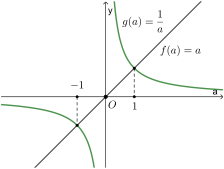
\includegraphics[scale=1]{2020-1129-0950-crop}
    \end{center}
    
    方法三: 也可以将不等式化为 $a-\dfrac1a>0$, 令 $h(a)= a-\dfrac1a$, 再作图求解. 只需留意函数 $h(a)$ 在 $(-\infty,0)$ 和 $(0,+\infty)$ 上均单调递增, 且与横轴的交点为 $(-1,0)$ 和 $(1,0)$ (参考 ``2020 年 11 月 8 日答疑记录''的例~\ref{exa:201206-1410}).
\end{solution}

\begin{remark}
    (1) 例~\ref{exa:201129-0950} 的方法一是代数解法, 变形后的式子 $(a^2-1)a>0$ 是三次不等式, 仍需要分类讨论, 各自求解后再取并集.
    
    (2) 方法二和方法三均利用了函数图形 (前者两个, 后者一个), 用这种方法时需要根据题意构造容易画出大致图形的函数, 也就是要事先了解函数的特点 (单调性、奇偶性、对称性、与坐标轴的交点, 等等).
\end{remark}

\begin{example}\label{exa:201129-1010}
    设定义在 $(-1,1)$ 上的奇函数 $f(x)$ 是增函数, 且 $f(a)+f(2a-1)<0$, 求 $a$ 的取值范围.
\end{example}
\begin{solution}
    因为 $f(x)$ 是奇函数, 所以不等式化为 
    \[f(a)< -f(2a-1)=f(1-2a).\]
    结合 $f(x)$ 是定义在 $(-1,1)$ 上的增函数知
    \[\left\{\!\!\begin{array}{l}
        -1<a<1,\\
        -1<1-2a<1,\\
        a<1-2a,
        \end{array}\right.\ \text{解得}\quad
      0<a<\frac13,\]
    即 $a\in\biggl(0,\dfrac13\biggr)$.
\end{solution}

例~\ref{exa:201129-1010} 中主要利用 ``$f(x)$ 是增函数'' 将抽象的不等式 (没有具体解析式的不等式) 
\[f(a)< f(1-2a)\]
化为具体的不等式 
\[a<1-2a.\]
再如, 若 $f(x)$ 是减函数, 则由 $f(a)< f(2a+1)$ 可知 $a>2a+1$. 在去掉 ``$f$'' 时, 也需要注意 $f$ 的作用范围 (即题中 $f(x)$ 的定义域).

\subsection{对数练习}

对数的主要运算法则如下 (以下均设底数 $a\in(0,1)\cup(1,+\infty)$, 真数 $x$, $y>0$):
\[\begin{gathered}
    a^x=y\Leftrightarrow x=\log_a y,\quad \text{由此可得}\ 
        a^{\log_a y}= y,\ x= \log_a a^x,\\
    \log_a x+ \log_a y= \log_a xy,\quad 
        \log_a x- \log_a y= \log_a \dfrac{x}y,\\
    \frac{\log_a x}{\log_a y}= \log_y x\ (\text{换底公式}),\quad
        \log_a x^\beta= \beta\log_a x\ (\beta\in\realnum). 
\end{gathered}\]
以上公式均可以逆用, 如 
\[\log_2 6= \log_2 2+\log_2 3= 1+\log_2 3.\]
此外还应注意恒等式 $\log_a a=1$ 和 $\log_a 1= 0$ (均由对数定义可得). 有两个取特殊底的对数是常用的: $\log_{10} x$ 记为 $\lg x$ (\myindex{常用对数}{常用对数}), $\log_{\mathrm{e}} x$ 记为 $\ln x$ (\myindex{自然对数}{自然对数}), 其中 $\mathrm{e}= 2.718\cdots$ 称为自然对数的底数.

\begin{example}
    对数练习:
    \begin{fourcolpro}
        (1) $\lg 0.0001$; & (2) $\log_2 6- \log_2 3$;
            & (3) $\ln \sqrt{\mathrm{e}}$; 
            & (4) $\log_3 5-\log_3 15$;\\
        (5) $\lg\dfrac14- \lg25$; & (6) $\log_2(\log_2 16)$;
            & \multicolumn{2}{l}{(7) $(\log_4 3+ \log_8 3)
            (\log_3 2+\log_9 2)$.}
    \end{fourcolpro}
\end{example}
\begin{solution}
    (1) $\lg 0.0001= \lg 10^{-4}= -4$ (注意 $0.1=\dfrac1{10}= 10^{-1}$).
    
    (2) $\log_2 6- \log_2 3= \log_2 \dfrac63= \log_2 2= 1$.
    
    (3) $\ln \sqrt{\mathrm{e}}= \ln \mathrm{e}^{\frac12}= \dfrac12$. 
    
    (4) $\log_3 5-\log_3 15= \log_3 \dfrac{5}{15}= \log_3 \dfrac13= -1$.
    
    (5) $\lg\dfrac14- \lg25= \lg\dfrac1{100}= -2$.
    
    (6) $\log_2(\log_2 16)= \log_2 4= 2$.
    
    (7) 由换底公式 (不妨均化为自然对数),
    \[\begin{aligned}
           &(\log_4 3+ \log_8 3)(\log_3 2+\log_9 2)\\
        ={}& \biggl(\frac{\ln 3}{\ln 4}+ \frac{\ln 3}{\ln 8}\biggr)
            \biggl(\frac{\ln 2}{\ln 3}+ \frac{\ln 2}{\ln 9}\biggr)\\
        ={}& \biggl(\frac{\ln 3}{2\ln 2}+ \frac{\ln 3}{3\ln 2}\biggr)
            \biggl(\frac{\ln 2}{\ln 3}+ \frac{\ln 2}{2\ln 3}\biggr)\\
        ={}& \biggl(\frac12+\frac13\biggr)\frac{\ln 3}{\ln 2}
            \biggl(1+\frac12\biggr)\frac{\ln 2}{\ln 3}\\
        ={}& \frac56\cdot\frac32
            = \frac54.
    \end{aligned}\]
\end{solution}
